%
% exemplo genérico de uso da classe iiufrgs.cls
% $Id: iiufrgs.tex,v 1.1.1.1 2005/01/18 23:54:42 avila Exp $
%
% This is an example file and is hereby explicitly put in the
% public domain.
%
\documentclass[ppgc,diss,english]{iiufrgs}
% Para usar o modelo, deve-se informar o programa e o tipo de documento.
% Programas :
%   * cic       -- Graduação em Ciência da Computação
%   * ecp       -- Graduação em Ciência da Computação
%   * ppgc      -- Programa de Pós Graduação em Computação
%   * pgmigro   -- Programa de Pós Graduação em Microeletrônica
%   
% Tipos de Documento:
%   * tc                -- Trabalhos de Conclusão (apenas cic e ecp)
%   * diss ou mestrado  -- Dissertações de Mestrado (ppgc e pgmicro)
%   * tese ou doutorado -- Teses de Doutorado (ppgc e pgmicro)
%   * ti                -- Trabalho Individual (ppgc e pgmicro)
% 
% Outras Opções:
%   * english    -- para textos em inglês
%   * openright  -- Força início de capítulos em páginas ímpares (padrão da
%                   biblioteca)
%   * oneside    -- Desliga frente-e-verso
%   * nominatalocal -- Lê os dados da nominata do arquivo nominatalocal.def


% Use unicode
\usepackage[utf8]{inputenc}   % pacote para acentuação

% Necessário para incluir figuras
\usepackage{mathtools}          % for \DeclarePairedDelimiter
\DeclarePairedDelimiter{\floor}{\lfloor}{\rfloor}
\usepackage{graphicx}           % pacote para importar figuras
\usepackage{Sweave}


\usepackage{times}              % pacote para usar fonte Adobe Times
% \usepackage{palatino}
% \usepackage{mathptmx}          % p/ usar fonte Adobe Times nas fórmulas

\usepackage[alf,abnt-emphasize=bf]{abntex2cite}	% pacote para usar citações abnt

%
% Informações gerais
%
\title{The Unbounded Knapsack Problem: a critical review}

\author{Becker}{Henrique}

% orientador e co-orientador são opcionais (não diga isso pra eles :))
\advisor[Prof.~Dr.]{Buriol}{Luciana}
%\coadvisor[Prof.~Dr.]{Knuth}{Donald Ervin}

% a data deve ser a da defesa; se nao especificada, são gerados
% mes e ano correntes
%\date{maio}{2001}

% o local de realização do trabalho pode ser especificado (ex. para TCs)
% com o comando \location:
%\location{Itaquaquecetuba}{SP}

% itens individuais da nominata podem ser redefinidos com os comandos
% abaixo:
% \renewcommand{\nominataReit}{Prof\textsuperscript{a}.~Wrana Maria Panizzi}
% \renewcommand{\nominataReitname}{Reitora}
% \renewcommand{\nominataPRE}{Prof.~Jos{\'e} Carlos Ferraz Hennemann}
% \renewcommand{\nominataPREname}{Pr{\'o}-Reitor de Ensino}
% \renewcommand{\nominataPRAPG}{Prof\textsuperscript{a}.~Joc{\'e}lia Grazia}
% \renewcommand{\nominataPRAPGname}{Pr{\'o}-Reitora Adjunta de P{\'o}s-Gradua{\c{c}}{\~a}o}
% \renewcommand{\nominataDir}{Prof.~Philippe Olivier Alexandre Navaux}
% \renewcommand{\nominataDirname}{Diretor do Instituto de Inform{\'a}tica}
% \renewcommand{\nominataCoord}{Prof.~Carlos Alberto Heuser}
% \renewcommand{\nominataCoordname}{Coordenador do PPGC}
% \renewcommand{\nominataBibchefe}{Beatriz Regina Bastos Haro}
% \renewcommand{\nominataBibchefename}{Bibliotec{\'a}ria-chefe do Instituto de Inform{\'a}tica}
% \renewcommand{\nominataChefeINA}{Prof.~Jos{\'e} Valdeni de Lima}
% \renewcommand{\nominataChefeINAname}{Chefe do \deptINA}
% \renewcommand{\nominataChefeINT}{Prof.~Leila Ribeiro}
% \renewcommand{\nominataChefeINTname}{Chefe do \deptINT}

% A seguir são apresentados comandos específicos para alguns
% tipos de documentos.

% Relatório de Pesquisa [rp]:
% \rp{123}             % numero do rp
% \financ{CNPq, CAPES} % orgaos financiadores

% Trabalho Individual [ti]:
% \ti{123}     % numero do TI
% \ti[II]{456} % no caso de ser o segundo TI

% Monografias de Especialização [espec]:
% \espec{Redes e Sistemas Distribuídos}      % nome do curso
% \coord[Profa.~Dra.]{Weber}{Taisy da Silva} % coordenador do curso
% \dept{INA}                                 % departamento relacionado

%
% palavras-chave
% iniciar todas com letras minúsculas, exceto no caso de abreviaturas
%
\keyword{unbounded knapsack problem}
\keyword{dynamic programming}
\keyword{optimization}
\keyword{cutting stock problem}

%
% inicio do documento
%
\begin{document}


% folha de rosto
% às vezes é necessário redefinir algum comando logo antes de produzir
% a folha de rosto:
% \renewcommand{\coordname}{Coordenadora do Curso}
\maketitle

% dedicatoria
\clearpage
\begin{flushright}
\mbox{}\vfill
{\sffamily\itshape
``If I have seen farther than others,\\
it is because I stood on the shoulders of giants.''\\}
--- \textsc{Sir~Isaac Newton}
\end{flushright}

% agradecimentos
\chapter*{Agradecimentos}

\begin{abstract}
The abstract can't be more than 500 words long.
\end{abstract}

% Ironically, this is the brazilian portuguese abstract if the dissertation
% is written in english.
\begin{englishabstract}{O problema da mochila com repetições: uma revisão crítica}{problema da mochila com repetições, programação dinâmica, otimização, cutting stock problem}
O resumo não deve conter mais que 500 palavras.
\end{englishabstract}

% lista de abreviaturas e siglas
% o parametro deve ser a abreviatura mais longa
\begin{listofabbrv}{IEACDA}
        \item[UKP] Unbounded Knapsack Problem
        \item[B\&B] Branch and Bound
        \item[DP] Dynamic Programming
        \item[PRNG] Pseudo-Random Number Generator
        \item[CSP] Cutting Stock Problem
        \item[BPP] Bin Packing Problem
	\item[IEACDA] Integer Equivalent Aggregation and Consistency Determination Approach
\end{listofabbrv}

% idem para a lista de símbolos
\begin{listofsymbols}{$\alpha\beta\pi\omega$}
       \item[$\sum{\frac{a}{b}}$] Somatório do produtório
       \item[$\alpha\beta\pi\omega$] Fator de inconstância do resultado
\end{listofsymbols}

% lista de figuras
\listoffigures

% lista de tabelas
\listoftables

% sumario
\tableofcontents

% aqui comeca o texto propriamente dito

% to make latex see the pdfs created by Sweave
\graphicspath{{chapters/}}
\chapter{The instance classes}

%final
If the author of this work could suggest one single thing to be improved in the future works about UKP, it would be the selection of the instances.

%working
The UKP is a variation of the classic knapsack problem, with the difference that an unbounded number of each item is available.

The study of the UKP has fallen in one of the pitfalls described by David Johnson in his guide to 

%pending
the ukp seems like a problem that should have many applications, but <CITE PYAsUKP 'are hard to find'>
the most classical real-world use of the problem is the unidimensional cutting stock problem 
	explain the problem
	explain how branch and price can be used to solve the problem
	cite gilmore and gomory (and brevily point that UKP5 and ordered step-off are very similar, more will be said in the algorithms section)
point error in the article, the pure UKP can only be used to solve the root node of the cutting stock exact continuous relaxation
the best solver don't use UKP anymore at all, but one of the good solvers use it, and repoted that in some cases, about 70\% of the processing is done at the root node

the use of artificial instances was already strongly crticized in the past
the reasons for their use is the possibility of generating many instances, of many sizes (what allows for examinating the growth of the time with the growth of the instance)
	This is specially interesting for UKP because it's one of the easiest NP-Hard problems, so big instances or hard instances have to be used to get high execution times, small execution times are too much affected by variance
	yet, artificial instances should not be used at all, if there's no guarantee that the growth/time/results will translate for real world instances (i.e. artificial instances should follow )

	The paper are the hard knapsack problems shows that even for 0-1 knapsack instances (that are by default harder than UKP instances), the instances used were easy to solve


The major problem with an experimental analysis of the UKP solving methods over artificial instances is that the different solving approaches are affected by the items distributions (i.e. some methods are the best for some for some distributions and the worst for others). Consequently, the results aren't useful for someone that wants to tackle real world UKP instances, unless some artificial instance distribution ends up modelling the 

TODO: The use of testbeds is overrated?

We have already pointed (TODO: refer to timeline) that the choices of item distributions on the generation of artificial instances in the previous literature has defined what was considered the best algorithm. I have written two sections of this chapter to further illustrate this point. Those are sections are (TODO: refer to) uncorrelated instances, and the second is the BREQD instances. The former points (TODO: list things pointed in uncorrelated instances); the latter presents a new instance distribution, that's easy to solve by B\&B methods and hard to solve by DP methods (some experimental results over this classes of instances will be presented at TODO: refer).

\section{Uncorrelated Random Coeficients Instances}

In this work, the expression `uncorrelated instances' will be used to refer to a family of UKP instances where the weight and the profit of an item have no correlation. The most common way for generating those uncorrelated instances is generating a value between \(w_{min}\) and \(w_{max}\) for the weight, and a value between \(p_{min}\) and \(p_{max}\) for the profit, for each of the \(n\) items of the instance using a (pseudo-)random number generator with an uniform distribution. %Uncorrelated instances can be generated using a (pseudo-)random number generator to generate \(n\) numbers between \(w_{min}\) and \(w_{max}\), and another \(n\) numbers between \(p_{min}\) and \(p_{max}\). Sorting both arrays will give (TODO: refer to realistic instances), that is another instance type. Uncorrelated instances 

PUTS IMAGE
\begin{figure}
    \caption{An uncorrelated instance generated with \(n = 100\), \(w_{min} = 1\), \(w_{min} = 1000\), \(p_{min} = 1\), and \(p_{max} = 1000\).}
    \begin{center}
    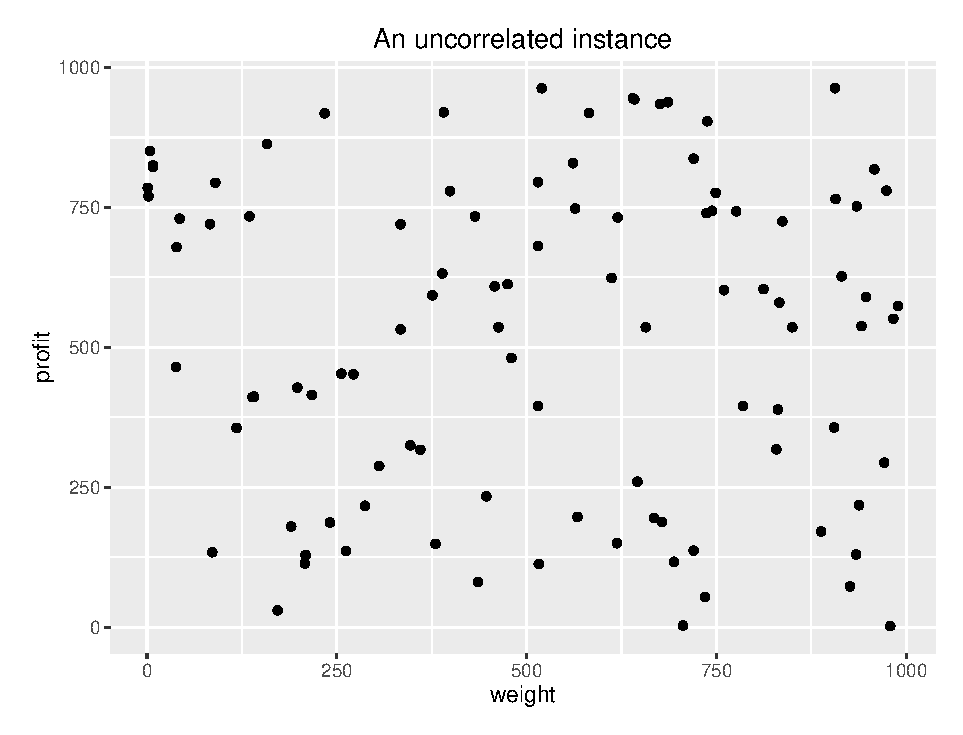
\includegraphics[scale=1]{uncorrelated.eps}
    \end{center}
    \legend{Source: the author.}
    \label{fig:uncorrelated_example}
\end{figure}

Expose why they are uninteresting: we do not know if they model any real world instance; it's a simple matter of running a good polynomial simple/multiple dominance algorithm first, or using MTU2 that was developed for this purpose. Increasing values of \(n\) increase the time taken by MTU2 or dominance removal in a polynomial fashion. The NP-hard part of the problem, that is finding an optimal solution between non-dominated items don't grow with \(n\). %(sorting or the \(O(n^2)\) dominance algorithms).

\section{Bottom Right Ellipse Quadrant Instances}

The Bottom Right Ellipse Quadrant Instances (`BREQ instances', for short) is a new UKP instance item distribution proposed by the author in this work. This instance distribution was created to illustrate that different item distributions favor different solution approaches and, therefore, the choice of instances (or specifically, their item distribution) defines what is considered the `best algorithm'.

Distributions that are easy to solve by the DP approach and hard to solve by the B\&B approach are common in the literature. This distribution has the opposite characteristic, it is hard to solve by DP and easy to solve by B\&B. It's important to point that this is an artificially generated distribution that don't model any real world instances (that the author have knowledge). The author discourages the use and study of such artificial instances, and created this distribution only as a tool to demonstrate that isn't hard to create a distribution that benefits a solving approach over another. It's the author's opinion that research should focus on real-world instances and/or artificially generated instances that clearly model real world instances.

The name given to this distribution is derived from the fact that, when plotted on a graph, the items show the form of a quarter of ellipse (specifically, the bottom right quadrant). All items in such distribution respect the following equation: \(p_i = p_{max} - \floor[\big]{\sqrt{p_{max}^2 - (w_i^2 \times \frac{p_{max}}{w_{max}}^2)}}\)\footnote{In this context, \(w_{max}\) and \(p_{max}\) define the quadrant top right corner, i.e. the possible maximum value for an item's weight and profit, an item with those exact values doesn't need to exist in a BREQ instance. The rounding down in the formulae can be dropped if the profit is a real number and not an integer.}. A natural consequence of this distribution shape is that the item profit grows quadratically with the item weight. This leads to the inexistance of simple, multiple and collective dominance\footnote{In truth, if the profit is integer, the smallest items can display some of those three dominances because the profit precision loss by rounding, but this is of little relevance and can be safely ignored for most purposes. If profit is an infinite precision real, the statement has no exceptions.}. In other words, for any multiset of items \(s\) and any single item \(i\) (with respective weigths \(w_s\) and \(w_t\), and respective profits \(p_t\) and \(p_i\)), if \(w_s \leq w_i\) then \(p_s < p_i\).

On the other hand, threshold dominance is very common in this instance type. With exception of the best item, any item of any instance (of any distribution) will always be threshold dominated at some capacity. However, in many instances the knapsack capacity is smaller than those threshold values and therefore the threshold dominance isn't applied or relevant. On BREQ instances, as a consequence of the quadratic profit growth, an optimal solution will never include the item \(i\) two or more times if there's an item \(j\) such as that \(\sqrt{2} \times w_i < w_j \leq 2 \times w_i\); so each item have a good probability of being threshold dominated before the second use. 

The solutions of BREQ instances will often contain the maximum number of copies of the largest item (that is also the most profitable, and the most efficient) allowed by the instance capacity. Any gap left will probably be filled by the heaviest item that fits the gap, with this process repeated until no item fits the gap left. A greedy heuristic procedure that followed those steps would probably yield an optimal solution. However, this is not always the case\footnote{A counter-example follows: consider an instance with \(n = 4\), \(c = 512\), \(w_1 = 384\), \(p_1 = 2774\), \(w_2 = 383\), \(p_2 = 2756\), \(w_3 = 129\), \(p_3 = 265\), \(w_4 = 32\) and \(p_4 = 17\); the optimal solution don't use the best item (\(w_1, p_1\)); the best solution when using the best item has a profit value of \(2842 = 2774 + 4\times17\) (weight \(512 = 384 + 4\times32\)) while the best solution when using the second most efficient item has the optimal profit value of \(3021 = 2756 + 265\) (weight \(512 = 383 + 129\)). In this case, between two solutions with the same weight, the one with the best item isn't the best one. The weight and profit values of this example follow the a BREQ distribution with \(w_{max} = 512\) and \(p_{max} = 8192\).}.

Our objective is not explore this distribution and its behaviour with different paremeters. Therefore, from now on we will refer only to instances with \(p_{min} = w_{min} = 1\) and \(w_{max} = c\). 

\section{Uncorrelated Random Coeficients Instances}

\section{Chung}
% TEX COPIED FROM SEA 2016 article, CHANGE AND AMPLIFY

\section{PYAsUKP instances}

This section will discuss the instance sets used in~\cite{pya}.
The distributions used by the instances weren't novel, but a 
Those instance sets were artificially generated with the purpose of being ``hard to solve'', what means a different thing for each one of them.


The same tool was used to generate the datasets (PYAsUKP), and the same parameters were used, otherwise noted the contrary. 
In Subsection 5.1.1 \emph{Known ``hard'' instances} of~\cite{pya} some sets of easy instances are used to allow comparison with MTU2. 
However, the authors reported integer overflow problems with MTU2 on harder instances. 
With exception of the subset-sum dataset, all datasets have a similar harder set (Subsection 5.2.1 \emph{New hard UKP instances}~\cite{pya}).
Thus, we considered in the runs only the harder ones. 
Each instance has a random capacity value within intervals shown in Table~\ref{tab:times}. 
The PYAsUKP parameters \mbox{\emph{-wmin \(w_{min}\) -cap c -n \textbf{n}}} were used in all instances generation. 
%When we found a discrepancy between the formula presented in \cite{pya} and the PYAsUKP code, or generated instances, we opted for changing the formula based on the observed behavior. 
%As our knowledge of OCaml is limited, we cannot guarantee that the formula presented here is a perfect match for the code; but, based by the generated instances, we believe it to be correct to a good extent.
We found some small discrepancies between the formulas presented in~\cite{pya} and the ones used in PYAsUKP code.
We opted for using the ones from  PYAsUKP code, and they are presented below.

\subsubsection{Subset-Sum}\label{sec:subsetsum}
Instances generated with \(p_i = w_i = rand(w_{min}, w_{max})\). 
The majority of the subset-sum instances used in \cite{pya} were solved on less than a centisecond in our experiments. 
This makes it easy to have imprecise measuring. 
Because of this, in this paper, we use a similar dataset, but with each parameter multiplied by ten. 
Therefore, we generated 10 instances for each possible combination of: \(w_{min} \in \{10^3, 5\times10^3, 10^4, 5\times10^4, 10^5\}\); \(w_{max} \in \{5\times10^5, 10^6\}\) and \(n \in \{10^3, 2\times10^3, 5\times10^3, 10^4\}\), totaling 400 instances. We do not discriminate each combination in~Table \ref{tab:times} for brevity. The PYAsUKP \emph{-form ss -wmax \(w_{max}\)} parameters were used.

\subsubsection{Strong Correlation}
Instances generated using the following formula: \(w_i = w_{min} + i - 1\) and \(p_i = w_i + \alpha\), for a given \(w_{min}\) and \(\alpha\).  Note that, except by the random capacity, all instances with the same \(\alpha\), \(\mathbf{n}\), and \(w_{min}\) combination are equal. The formula doesn't rely on random numbers. The PYAsUKP \emph{-form chung -step \(\alpha\) } parameters were used.

\subsubsection{Postponed Periodicity}
This family of instances is generated by the following method: \textbf{n} distinct weights are generated with \(rand(w_{min}, w_{max})\) and then sorted by increasing order; \(p_1 = w_1 + rand(1, 500)\); and \(\forall i \in [2, n].~p_i = p_{i-1} + rand(1, 125)\). The \(w_{max}\) is computed as \(10\overline{n}\). The PYAsUKP \emph{-form nsds2 -step 500 -wmax \(w_{max}\)} parameters were used.

\subsubsection{No Collective Dominance}
This family of instances is generated by the following method: \textbf{n} distinct weights are generated with \(rand(w_{min}, w_{max})\) and then sorted by increasing order; \(p_1 = p_{min} + rand(0, 49)\); and \(\forall i \in [2, n].~p_i = \lfloor w_i \times ((p_{i-1}/w_{i-1}) + 0.01)\rfloor + rand(1, 10)\). The given values are: \(w_{min} = p_{min} = \mathbf{n}\) and \(w_{max} = 10\overline{n}\). The PYAsUKP \emph{-form hi -pmin \(p_{min}\) -wmax \(w_{max}\)} parameters were used.

\subsubsection{SAW}
This family of instances is generated by the following method: generate \textbf{n} random weights between \(w_{min}\) and \(w_{max} = 1\overline{n}\) with the following property: \(\forall i \in [2, n].~w_i~mod~w_1 > 0\) (\(w_1\) is the smallest weight); sort by increasing order; then \(p_1 = w_1 + \alpha\) where \(\alpha = rand(1,5)\), and \(\forall i \in [2, n].~p_i = rand(l_i, u_i)\) where \(l_i = max(p_{i-1}, q_i)\), \(u_i = q_i + m_i\), \(q_i = p_1 \times \lfloor w_i / w_1 \rfloor \), and \(m_i = w_i~mod~w_1\). The PYAsUKP \emph{-form saw -step \(\alpha\) -wmax \(w_{max}\)} parameters were used.

% maybe this goes in another section
	timeline: DP -> huge random instances -> B\&B is better (no empiric evidence) -> instances that are hard for B\&B (linear distribution) -> PYAsUKP is better than B\&B in instances designed to be hard to solve by it (in fact any DP non-naive DP solution would have results better than B\&B methods only, like MTU1 and MTU2). also, using MTU2 instead of MTU1 shows a lack of understanding of the methods. MTU2 was developed for very large random instances, not for relatively small and hard (distribution-wise) instances



% introducao
\chapter{Introdução}
No início dos tempos, Donald E. Knuth criou o \TeX. Algum tempo depois, Leslie Lamport criou o \LaTeX. Graças a eles, não somos obrigados a usar o Word nem o LibreOffice.

\section{Figuras e tabelas}

Esta seção faz referência às Figuras~\ref{fig:estrutura},~\ref{fig:ex1} e~\ref{fig:ex2}, a título de exemplo. A primeira figura apresenta a estrutura de uma figura. A \emph{descrição} deve aparecer \textbf{acima} da figura. Abaixo da figura, deve ser indicado a origem da imagem, mesmo se essa for apenas os autores do texto.

A Figura~\ref{fig:ex1} representa o caso mais comum, onde a figura propriamente dita é importada de um arquivo (neste exemplo em formato \texttt{eps} ou \texttt{pdf}. Veja a seção \ref{sec:fig_format}). A Figura~\ref{fig:ex2} exemplifica o uso do environment \texttt{picture}, para desenhar usando o próprio~\LaTeX.

\begin{figure}[h]
    \caption{Descrição da Figura deve ir no topo}
    \begin{center}
        % Aqui vai um includegraphics , um picture environment ou qualquer
        % outro comando necessário para incorporar o formato de imagem
        % utilizado.
        \begin{picture}(100,100)
                \put(0,0){\line(0,1){100}}
                \put(0,0){\line(1,0){100}}
                \put(100,100){\line(0,-1){100}}
                \put(100,100){\line(-1,0){100}}
                \put(10,50){Uma Imagem}
        \end{picture}
    \end{center}
    \label{fig:estrutura}
    \legend{Fonte: Os Autores}
\end{figure}

\begin{figure}
    \caption{Exemplo de figura importada de um arquivo e também exemplo de caption muito grande que ocupa mais de uma linha na Lista~de~Figuras}
    \centerline{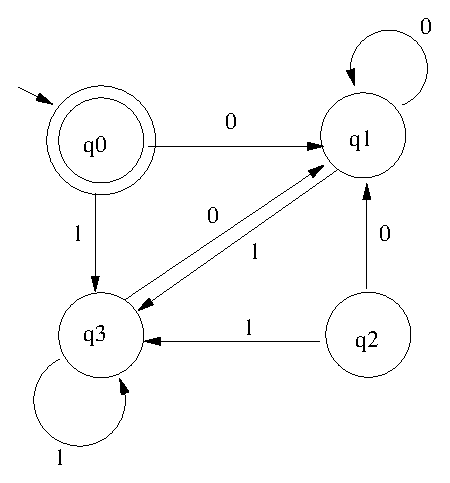
\includegraphics[width=8em]{fig}}
    \legend{Fonte: Os Autores}
    \label{fig:ex1}
\end{figure}

% o `[h]' abaixo é um parâmetro opcional que sugere que o LaTeX coloque a
% figura exatamente neste ponto do texto. Somente preocupe-se com esse tipo
% de formatação quando o texto estiver completamente pronto (uma frase a mais
% pode fazer o LaTeX mudar completamente de idéia sobre onde colocar as
% figuras e tabelas)
%\begin{figure}[h]
\begin{figure}
    \caption{Exemplo de figura desenhada com o environment \texttt{picture}.}
    \begin{center}
        \setlength{\unitlength}{.1em}
        \begin{picture}(100,100)
                \put(20,20){\circle{20}}
                \put(20,20){\small\makebox(0,0){a}}
                \put(80,80){\circle{20}}
                \put(80,80){\small\makebox(0,0){b}}
                \put(28,28){\vector(1,1){44}}
        \end{picture}
    \end{center}
    \legend{Fonte: Os Autores}
    \label{fig:ex2}
\end{figure}

Tabelas são construídas com praticamente os mesmos comandos. Ver a tabela \ref{tbl:ex1}.

\begin{table}[h]
    \caption{Uma tabela de Exemplo}
    \begin{center}
        \begin{tabular}{c|c|p{5cm}}
            \textit{Col 1}  &   \textit{Col 2}  &   \textit{Col 3} \\
            \hline
            \hline
            Val 1           &   Val 2           & Esta coluna funciona como um parágrafo, tendo uma margem definida em 5cm. Quebras de linha funcionam como em qualquer parágrafo do tex. \\
            Valor Longo     & Val 2             & Val 3 \\
            \hline
        \end{tabular}
    \end{center}
    \legend{Fonte: Os Autores}
    \label{tbl:ex1}
\end{table}

\subsection{Formato de Figuras}
\label{sec:fig_format}

O LaTeX permite utilizar vários formatos de figuras, entre eles \emph{eps}, \emph{pdf}, \emph{jpeg} e \emph{png}. Programas de diagramação como Inkscape (e mesmo LibreOffice) permitem gerar arquivos de imagens vetoriais que podem ser utilizados pelo LaTeX sem dificuldade. Pacotes externos permitem utilizar SVG e outros formatos.

Dia e xfig são programas utilizados por dinossauros para gerar figuras vetoriais. Se possível, evite-os.

\subsection{Classificação dos etc.}

O formato adotado pela ABNT prevê apenas três níveis (capítulo, seção e subseção). Assim, \texttt{\char'134subsubsection} não é aconselhado.

\section{Sobre as referências bibliográficas}

A classe \emph{iiufrgs} faz uso do pacote \emph{abnTeX2} com algumas alterações
feitas por Sandro Rama Fiorini. Culpe ele se algo der errado. Agradeça a ele
pelo que der certo. As modificações dão uma camada de tinta NATBIB-style,
já que o abntex2 usa uns comandos de citação feitos para alienígenas de 5 braços 
wtf. Exemplos de citação:

\begin{itemize}
    \item \emph{cite}: Unicórnios são verdes \cite{Adams2009Conceptual};
    \item \emph{cite}:Unicórnios são verdes \cite{Adams2009Conceptual};
    \item \emph{cite}: Segundo \cite{Adams2009Conceptual}, unicórnios são
                        verdes.
    \item \emph{citen or citenum}: Segundo \cite{Adams2009Conceptual},
        unicórnios são verdes.
    \item \emph{citeauthor e citeyearpar}: Segundo artigos de
        \cite{Adams2009Conceptual} , unicórnios são verdes 
        \cite{Adams2009Conceptual}.

\end{itemize}

O estilo abnt fornecido antigamente pelo UTUG não é mais recomendado, pois não
produz saída de acordo com as exigências da biblioteca.

Recomenda-se o uso de bibtex para gerenciar as referências (veja o arquivo
biblio.bib).

% e aqui vai a parte principal
%
% \chapter{Estado da arte}
% \chapter{Mais estado da arte}
% \chapter{A minha contribuição}
% \chapter{Prova de que a minha contribuição é válida}
% \chapter{Conclusão}

% referencias
% aqui será usado o environment padrao `thebibliography'; porém, sugere-se
% seriamente o uso de BibTeX e do estilo abnt.bst (veja na página do
% UTUG)
%
% observe também o estilo meio estranho de alguns labels; isso é
% devido ao uso do pacote `natbib', que permite fazer citações de
% autores, ano, e diversas combinações desses

\bibliographystyle{abntex2-alf}
\bibliography{biblio}

\end{document}
